\documentclass{article}
\usepackage[%
    left=0.5in,%
    right=0.5in,%
    top=0.5in,%
    bottom=0.5in,%
]{geometry}%
\usepackage{minitoc}
\usepackage{multicol}
\usepackage{graphicx}
\usepackage{fixltx2e}
\usepackage{listings}
\usepackage{color}
\usepackage{hyperref}
    \hypersetup{ colorlinks = true, linkcolor = blue }
\usepackage{blindtext}
\definecolor{lightgray}{gray}{0.9}
\graphicspath{ {./} }


\newcommand{\inlinecode}[2]{\colorbox{lightgray}{\lstinline
[language=#1]$#2$}}
\newcommand{\worddef}[1]{\hyperref[sec:reference]{\textit{#1}}}

\begin{document}

\section{Definitions}

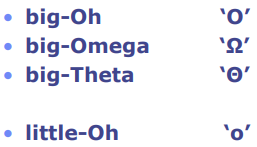
\includegraphics[scale=0.8]{Selection_003.png}
\subsection{Big-Omega}
\begin{flushleft}
Defintion: Given funciton $f(n)$ and $g(n)$, we say that\\
\ $ f(n)\ is\ \Omega(g(n))$\\
If there are (strictly) positive constants $c$ and $n_o$, such that\\
\ $ f(n) \geq c g(n)$ for all $ n \geq n_o$\\
Note that $ c > 0$ and $c$ must be \textbf{constant}(cannot depend on n)\\
Similarly to big-Oh, Big-Omega is: Reflexive, \textbf{NOT} symetric, transative.
\end{flushleft}

\subsection{Linking big-Oh and Big-Omega}


\pagebreak
\section*{Reference section} \label{sec:reference}
\begin{description}
	\item[placeholder] \hfill \\ placeholder
\end{description}
\end{document}
